\documentclass{article}
\usepackage[utf8]{inputenc}  
\usepackage[T1]{fontenc}     
\usepackage{graphicx}
\usepackage{amsmath}
\usepackage{pgfplots}
\usepackage{tikz}

\title{Sprawozdanie z zad nr 4}
\author{Jan Ryszkiewicz}
\date{\today}

\begin{document}

\maketitle

\section*{Zadanie 1: Nierówności ogonowe dla rozkładu dwumianowego \text{Bin}\left(n, \frac{1}{2}\right)}

Przybliżałem wartości następujących prawdopodobieństw za pomocą nierówności Markowa i Czebyszewa:
\begin{itemize}
    \item \( P\left(X \geq \frac{6}{5} \cdot \mathbb{E}(X)\right) \)
    \item \( P\left( \left| X - \mathbb{E}(X) \right| \geq \frac{1}{10} \cdot \mathbb{E}(X) \right) \)
\end{itemize}

\hspace*{-0cm} 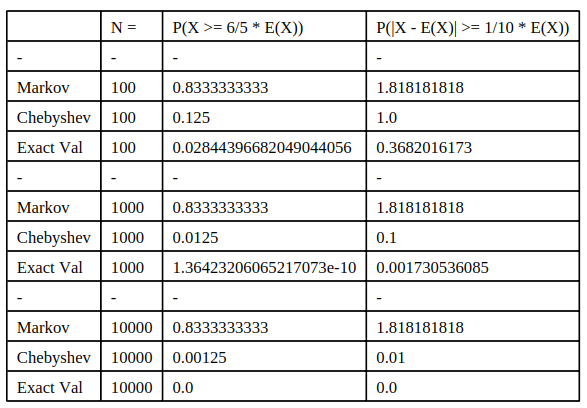
\includegraphics[scale=0.5]{./plots/exc1.png}

Po przeprowadzeniu obliczeń wyraźnie widać że nierówność Czebyszewa daje nieporównywalnie lepsze przybliżenie.
aczkolwiek nadal jest ono dalekie od dokładnego, co widać po różnicy od wartości faktycznej. \\

\section*{Zadanie 2: Błądzenie losowe na liczbach całkowitych}

\textit{interpretuję tutaj plik exc2.pdf}

wyraźnie widać że razem z rosnącym N dystrybuanta \( S_N \) jest coraz lepiej przybliżana przez \\
dystrybuantę rozkładu Normalnego standardowego, co jest zgodne z \textbf{CLT} \\

\section*{Zadanie 3: Błąadzenie losowe na \mathbb{Z} rozkład \textit{„czasu spęedzonego nad osią OX”}}

\textit{interpretuję tutaj plik exc3.pdf}

Z wykresów łatwo zauważyć, że w przeważającej ilości przypadków większość czasu spędzimy pod lub nad osią \( O_X \) a rzadko po środku\\
Sam wykres przypomina natomiast funkcję gęstości dla dystrybuanty = \\
\( \frac{2}{\pi} \arcsin\left(\sqrt{t}\right), \quad t \in [0, 1] etc. \)\\
(zad 5 lista 8)

\end{document}
